\chapter{Document Retrieval}

We are given a collection $D' = \{d_1, \ldots, d_{N-1}\}$ of documents. Each of $d_i$ is a string over an alphabet $\Sigma' = [2,\sigma]$ terminated by a sentinel symbol $1$ (or \#). We define $D = D' \cup d_0$ with a sentinel document $d_0 = 0$. We now want to answer word queries $Q = \{q_0, \ldots, q_{m-1}\}$. $Q$ is called \defi{bag of words}{Bag of Words} and is an unordered set of size $m$.

\begin{Definition}
  Given a collection $D$, a query $Q$ of length $m$ and a similarity measure $\mathcal{S} : D \times \mathcal{P}_{=m}(\Sigma') \to \mathbb{R}$. Calculate the \defi{top-k documents}{Top-k Documents} of $D$ with regard to $Q$ an $\mathcal{S}$.\newline
  That is a sorted list $T = \{\tau_0, \ldots, \tau_{k-1}\}$ with $\mathcal{S}(d_{\tau_i}, Q) \geq \mathcal{S}(d_{\tau_{i + 1}}, Q)$ for $0 \leq i < k$ and $\mathcal{S}(d_{\tau_{k-1}},Q) \geq \mathcal{S}(d_j, Q)$ for $j \not\in T$.
\end{Definition}

\section{Similarity Measures}

\begin{Definition}
  The following document dependent factors appear in many different similarity measures~$\mathcal{S}$:
  \begin{itemize}
    \item $f_{d,q}$ is the \defi{term frequency}{Term Frequency}. It counts the number of times, word $q$ appears in document~$d$.
    \item $F_{D,q}$ is the \defi{document frequency}{Document Frequency}. It counts the number of distinct documents from~$D$ containing~$q$ at least once.
  \end{itemize}
\end{Definition}

\begin{Definition}
  The \defi{Okapi BM25}{Okapi BM25} similarity measure is given by:
  \begin{align}
    \mathcal{S}_{Q,d}^{BM25} = \sum\limits_{q \in Q}
    \frac{\left(k_1 + 1\right)f_{d,q}}{k_1\left(1 - b + \frac{n_d}{n_{avg}}\right) + f_{d,q}}
    \cdot f_{Q,q} \cdot
    \ln\frac{N - F_{D,q} + 0.5}{F_{D,q} + 0.5}
  \end{align}
  Here $n_d$ is the length of document $d$ and $n_{avg}$ is the average document length.
\end{Definition}

There are several other possible ideas to build a similarity measure:
\begin{itemize}
  \item Documents can be assigned \defi{static weights}{Static Weighting}. An example is the Page-Rank algorithm.
  \item A \defi{language model}{Language Model} can be used to compute the probability to generate the query using the text statistics of each document.
  \item In a \defi{vector space model}{Vector Space Model} we compute the cosine of the angle in $\sigma$-dimensional space between a query vector and a document vector.
  \item \defi{Zone ranking}{Zone Ranking} weighs words appearing in the title of a web page weigh more than words in the body.
\end{itemize}

\section{Inverted Index}

\begin{Definition}
  In an \defi{inverted index}{Inverted Index} (IVI) for each term $q$ (excluding the sentinels) a list of pairs of document id and term frequency is stored. The pairs are ordered according to their document ids. Further for each term the document frequency is stored.
\end{Definition}

To process a query we sequentially iterate through the lists containing the query phrases and calculate the ranking function. The query complexity therefore depends on the document frequency.

It is not possible to answer phrase queries with this variant of an inverted index. Direct support of arbitrary phrase queries would require $\mathcal{O}(n^2)$ lists.

\begin{Example}
  Consider the three documents $\mathcal{D} = \{d_1, d_2, d_3\}$:
  \begin{align*}
    d_1 &: \text{is big data really big} \\
    d_2 &: \text{is it big in science} \\
    d_3 &: \text{big data is big}
  \end{align*}
  We will get the following inverted index:
  \begin{align*}
    \text{big} &: \{(1,2), (2,1), (3,2)\}  & F_{\mathcal{D}, \text{big}} = 3 \\
    \text{data} &: \{(1,1), (3,1)\} & F_{\mathcal{D}, \text{data}} = 2 \\
    \text{in} &: \{(2,1)\} & F_{\mathcal{D}, \text{in}} = 1 \\
    \text{is} &: \{(1,1), (2,1), (3,1)\} & F_{\mathcal{D}, \text{is}} = 3 \\
    \text{really} &: \{(1,1)\} & F_{\mathcal{D}, \text{really}} = 1 \\
    \text{science} &: \{(2,1)\} & F_{\mathcal{D}, \text{science}} = 1
  \end{align*}
\end{Example}

\begin{Theorem}
  An inverted index can be represented in $n\mathcal{H}_0(\mathcal{D}) + 3n + o(n) + \mathcal{O}(\sigma \log n)$ bits, where $n = \sum_{d \in \mathcal{D}} n_d$ and $f_{\mathcal{D},q} = \sum_{d \in \mathcal{D}} f_{d,q}$.
\end{Theorem}

\begin{Proof}
  For each term we use Elias-Fano-Encoding to store the increasing list of document ids. The list of frequencies itself is unary encoded decreased by one (each frequency~$x$ is encoded by~$x$ bits). With this representation we get:
  \begin{align}
    \begin{aligned}
      \proc{Space(IVI)}
      &\stackrel{\mathclap{\text{\ref{def:eliasDeltaEncoding}}}}{=}
      \sum\limits_{q \in \Sigma}
      \underbrace{2F_{\mathcal{D},q} + F_{\mathcal{D},q} \log\frac{N}{F_{\mathcal{D}, q}} + o(F_{\mathcal{D},q})}_{\text{document ids}} +
      \underbrace{f_{\mathcal{D},q}}_{\text{frequencies}} +
      \underbrace{\mathcal{O}(\log n)}_{\text{pointer}} \\
      &\leq 3n + o(n) + \mathcal{O}(\sigma \log n) + \sum\limits_{q \in \Sigma} F_{\mathcal{D},q}\log\frac{n}{F_{\mathcal{D},q}} \\
      &\stackrel{\mathclap{(*)}}{\leq}
      3n + o(n) + \mathcal{O}(\sigma \log n) +
      n\sum\limits_{q \in \Sigma}\frac{f_{\mathcal{D},q}}{n}\log\frac{n}{f_{\mathcal{D},q}} \\
      &= n\mathcal{H}_0(\mathcal{D}) + 3n + o(n) + \mathcal{O}(\sigma \log n)
    \end{aligned}
  \end{align}
  In $(*)$ we assumed that $f_{\mathcal{D},q} < \frac{n}{2}$ for all $q$. When the inverted index contains a sufficient amount of documents, this is safe to assume.
\end{Proof}

\section{GREEDY framework}

\begin{Definition}
  Let $\mathcal{D}$ be the \defi{document array}{Document Array} of length $n$. For each suffix $\id{SA}[i]$ the document array $\mathcal{D}[i]$ contains the identifier of the document, in which suffix $\id{SA}[i]$ starts. A suffix array (or suffix tree) with this information added is called \defi{generalized suffix array}{Generalized Suffix Array} (or \defi{generalized suffix tree}{Generalized Suffix Tree}).
\end{Definition}

\begin{Definition}
  The \defi{GREEDY framework}{GREEDY Framework} for single term $f_{d,q}$-ranking of Culpepper et al. \cite{Culpepper2010} consists of:
  \begin{itemize}
    \item A compressed suffix array \id{CSA} of concatenation $\mathcal{D}$.
    \item A wavelet tree of the document array of $D$.
  \end{itemize}
\end{Definition}

\section{Document Frequency $F_{\mathcal{D},q}$}

In this section we will see how to efficiently compute the document frequency $F_{\mathcal{D},q}$ for a given query $q$ following a method from Sadakane \cite{Sadakane2007}.

\begin{Definition}
  The \defi{binary generalized suffix tree}{Binary Generalized Suffix Tree} (\id{BGST}) of a text is the suffix tree with inserted inner nodes, such that the each vertex has degree $0$ or $2$. Figure~\ref{fig:binaryGeneralizedSuffixTreeExample} shows the \id{BGST} for \texttt{LA O LA \# O LA LA LA \# O O LA \# \$}.
\end{Definition}

To count the document frequency $F_{\mathcal{D},q}$, execute the following steps:
\begin{enumerate}
  \item Build the \id{BGST}.
  \item For each inner node $v$ in \id{BGST} keep a list $L_v$ of repeated documents. A document $d$ is added to $L_v$, if $d$ occurs in a leaf of the left and of the right subtree.
  \item For a pattern $q$ let $v_q$ be the \defi{locus}{Locus}, that is the lowest node which path is prefixed by $q$. $F_{\mathcal{D},q}$ equals the number of leaves in the subtree of $v_q$ minus the number of repeated documents ($\sum_{v \in T_{v_q}} \vert L_v \vert$) in $v_q$'s subtree $T_{v_q}$.
\end{enumerate}
To find the number of repeated documents in the subtree of an inner node, number the nodes in order (as in Figure~\ref{fig:binaryGeneralizedSuffixTreeExample}). Traverse in this order and append $\vert L_v \vert$ in unary coding ($\vert L_v \vert$ $0$s and one $1$) to a bitvector $H$, which was initialized with a single $1$. Then all nodes of each possible subtree are contiguous and the number of repeated documents can be calculated by two select queries. This is shown in Algorithm~\ref{alg:documentFrequency}. The runtime depends only on the time to do the backward search.

\begin{figure}[htb]
  \centering
  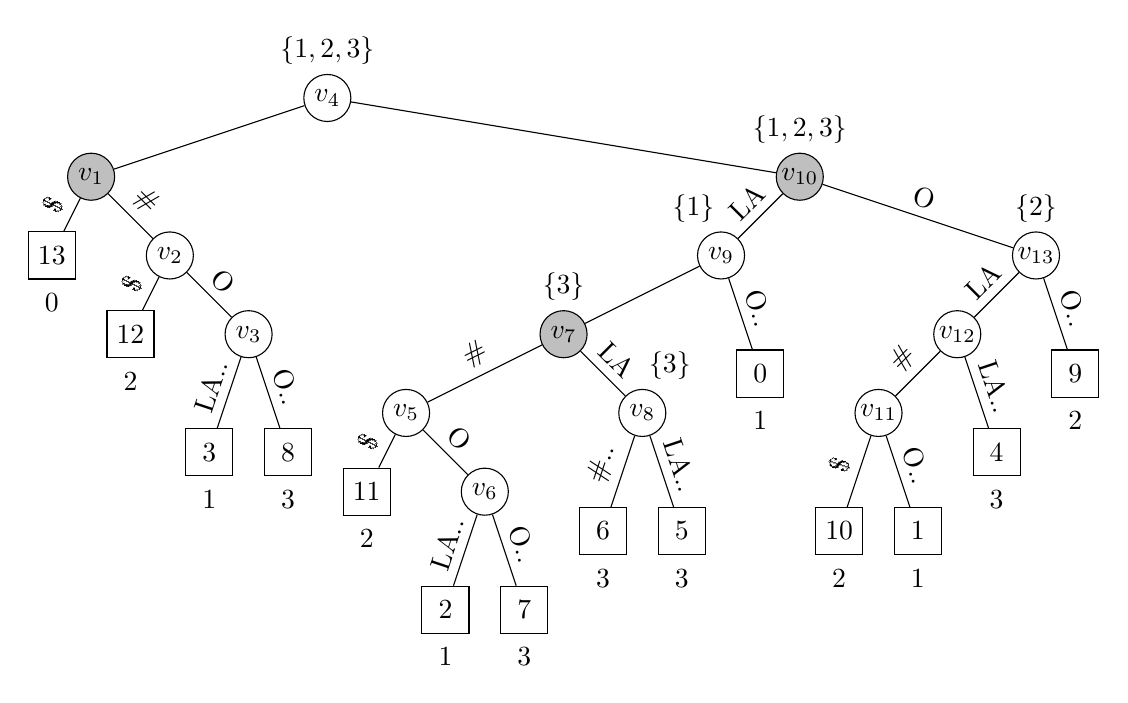
\begin{tikzpicture}[x={(5mm, 0mm)}]
  \tikzstyle{vertex}=[draw,minimum size=17pt, inner sep=0pt]
  \node[vertex, circle] (v4) at (0, 0) {$v_4$};
  \node (l4) at (0, 0.6) {$\{1,2,3\}$};

  \node[vertex, circle, fill=lightgray] (v1) at (-6, -1) {$v_1$};
  \draw (v4) -- (v1);

  \node[vertex, circle] (v2) at (-4, -2) {$v_2$};
  \draw (v1) -- (v2) node[above, sloped, pos=0.5] {\#};

  \node[vertex, circle] (v3) at (-2, -3) {$v_3$};
  \draw (v2) -- (v3) node[above, sloped, pos=0.5] {O};

  \node[vertex, circle, fill=lightgray] (v10) at (12, -1) {$v_{10}$};
  \node (l10) at (12, -0.4) {$\{1,2,3\}$};
  \draw (v4) -- (v10);

  \node[vertex, circle] (v9) at (10, -2) {$v_9$};
  \node (l9) at (9.3, -1.4) {$\{1\}$};
  \draw (v10) -- (v9) node[above, sloped, pos=0.5] {LA};

  \node[vertex, circle, fill=lightgray] (v7) at (6, -3) {$v_7$};
  \node (l7) at (6, -2.4) {$\{3\}$};
  \draw (v9) -- (v7);

  \node[vertex, circle] (v5) at (2, -4) {$v_5$};
  \draw (v7) -- (v5) node[above, sloped, pos=0.5] {\#};

  \node[vertex, circle] (v6) at (4, -5) {$v_6$};
  \draw (v5) -- (v6) node[above, sloped, pos=0.5] {O};

  \node[vertex, circle] (v8) at (8, -4) {$v_8$};
  \node (l8) at (8.7, -3.4) {$\{3\}$};
  \draw (v7) -- (v8) node[above, sloped, pos=0.5] {LA};

  \node[vertex, circle] (v13) at (18, -2) {$v_{13}$};
  \node (l13) at (18, -1.4) {$\{2\}$};
  \draw (v10) -- (v13) node[above, sloped, pos=0.5] {O};

  \node[vertex, circle] (v12) at (16, -3) {$v_{12}$};
  \draw (v13) -- (v12) node[above, sloped, pos=0.5] {LA};

  \node[vertex, circle] (v11) at (14, -4) {$v_{11}$};
  \draw (v12) -- (v11) node[above, sloped, pos=0.5] {\#};

  \node[vertex] (s13) at (-7, -2) {$13$};
  \node (d13) at (-7, -2.6) {$0$};
  \draw (v1) -- (s13) node[above, sloped, pos=0.5] {\$};

  \node[vertex] (s12) at (-5, -3) {$12$};
  \node (d12) at (-5, -3.6) {$2$};
  \draw (v2) -- (s12) node[above, sloped, pos=0.5] {\$};

  \node[vertex] (s3) at (-3, -4.5) {$3$};
  \node (d3) at (-3, -5.1) {$1$};
  \draw (v3) -- (s3) node[above, sloped, pos=0.5] {LA..};

  \node[vertex] (s8) at (-1, -4.5) {$8$};
  \node (d8) at (-1, -5.1) {$3$};
  \draw (v3) -- (s8) node[above, sloped, pos=0.5] {O..};

  \node[vertex] (s11) at (1, -5) {$11$};
  \node (d11) at (1, -5.6) {$2$};
  \draw (v5) -- (s11) node[above, sloped, pos=0.5] {\$};

  \node[vertex] (s2) at (3, -6.5) {$2$};
  \node (d2) at (3, -7.1) {$1$};
  \draw (v6) -- (s2) node[above, sloped, pos=0.5] {LA..};

  \node[vertex] (s7) at (5, -6.5) {$7$};
  \node (d7) at (5, -7.1) {$3$};
  \draw (v6) -- (s7) node[above, sloped, pos=0.5] {O..};

  \node[vertex] (s6) at (7, -5.5) {$6$};
  \node (d6) at (7, -6.1) {$3$};
  \draw (v8) -- (s6) node[above, sloped, pos=0.5] {\#..};

  \node[vertex] (s5) at (9, -5.5) {$5$};
  \node (d5) at (9, -6.1) {$3$};
  \draw (v8) -- (s5) node[above, sloped, pos=0.5] {LA..};

  \node[vertex] (s0) at (11, -3.5) {$0$};
  \node (d0) at (11, -4.1) {$1$};
  \draw (v9) -- (s0) node[above, sloped, pos=0.5] {O..};

  \node[vertex] (s9) at (19, -3.5) {$9$};
  \node (d9) at (19, -4.1) {$2$};
  \draw (v13) -- (s9) node[above, sloped, pos=0.5] {O..};

  \node[vertex] (s4) at (17, -4.5) {$4$};
  \node (d4) at (17, -5.1) {$3$};
  \draw (v12) -- (s4) node[above, sloped, pos=0.5] {LA..};

  \node[vertex] (s10) at (13, -5.5) {$10$};
  \node (d10) at (13, -6.1) {$2$};
  \draw (v11) -- (s10) node[above, sloped, pos=0.5] {\$};

  \node[vertex] (s1) at (15, -5.5) {$1$};
  \node (d1) at (15, -6.1) {$1$};
  \draw (v11) -- (s1) node[above, sloped, pos=0.5] {O..};
\end{tikzpicture}

  \caption{The binary generalized suffix tree of an example document collection $\mathcal{D} = \texttt{LA O LA \# O LA LA LA \# O O LA \# \$}$. The filled vertices are the dummy nodes added to get a binary tree. Round nodes are inner nodes, square nodes are leaves corresponding to suffixes. The number below each leaf is the entry in the document array.}
  \label{fig:binaryGeneralizedSuffixTreeExample}
\end{figure}

\begin{algorithm}[htb]
  \begin{codebox}
    \Procname{$\proc{Document-Frequency}(q)$}
    \li $[l,r] \gets \proc{Backward-Search(\id{CSA}, q)}$
    \li $s \gets r - l + 1$
    \li $y \gets \proc{Select}_1(r, H)$
    \li \If $l \isequal 0$
        \Then
    \li   \Return $s - (y - r + 1)$
    \li \Else
    \li   $x \gets \proc{Select}_1(l, H)$
    \li   \Return $s - (y - r + 1 - (x - l + 1))$
        \End
  \end{codebox}
  \caption{Compute the document frequency $F_{\mathcal{D},q}$ for query $q$.}
  \label{alg:documentFrequency}
\end{algorithm}

\begin{Example}
  Figure~\ref{fig:binaryGeneralizedSuffixTreeExample} shows the \id{BGST} for \texttt{LA O LA \# O LA LA LA \# O O LA \# \$}. We get the following bitvector $H$:
  \begin{align*}
    H = 1
    \underbrace{1}_{v_1}
    \underbrace{1}_{v_2}
    \underbrace{1}_{v_3}
    \underbrace{0001}_{v_4}
    \underbrace{1}_{v_5}
    \underbrace{1}_{v_6}
    \underbrace{01}_{v_7}
    \underbrace{01}_{v_8}
    \underbrace{01}_{v_9}
    \underbrace{0001}_{v_{10}}
    \underbrace{1}_{v_{11}}
    \underbrace{1}_{v_{12}}
    \underbrace{01}_{v_{13}}
  \end{align*}
  Let's now consider $q = \texttt{LA}$. Then \proc{Backward-Search} returns suffix array interval $[4,9]$. Executing the steps in Algorithm~\ref{alg:documentFrequency} yields $s = 6$, $y = 15$ and $x = 7$, so that $3$ is returned.
\end{Example}

\begin{Theorem}
  The document frequency can be calculated with an index needing $\mathcal{O}(n + \vert \id{CSA} \vert)$ bits space.
\end{Theorem}

\begin{Proof}
  The bitvector $H$ has maximum size $2n - N$. Additionally $o(n)$ bits for a constant time select structure are needed. The only thing left is the space needed for \id{CSA}.
\end{Proof}

\subsection{Calculating $F_{\mathcal{D}_v, q}$}

Let $F_{\mathcal{D}_v, q}$ be the subset of documents which are represented by a node in the wavelet tree over the document array. To compute it efficiently we introduce another array:

\begin{Definition}
  The \defi{repetition array}{Repetition Array} $R$ contains for each $0$ in $H$ the corresponding repeated element of the associated node.
\end{Definition}

We can build a wavelet tree \id{WTD} over the document array and a wavelet tree \id{WTR} over the repetition array. Using $\proc{Select}_1$ we can as above convert an interval $[l,r]$ of the suffix array into ranges in the two wavelet trees. When traversing \id{WTD} we can simultaneously traverse \id{WTR}. The size of the range in \id{WTR} always counts the number of repetitions.

\begin{Example}
  Continuing above example, we get for $H$ and $R$:
  \begin{align*}
    H &= 1
    \underbrace{1}_{v_1}
    \underbrace{1}_{v_2}
    \underbrace{1}_{v_3}
    \underbrace{0001}_{v_4}
    \underbrace{1}_{v_5}
    \underbrace{1}_{v_6}
    \underbrace{01}_{v_7}
    \underbrace{01}_{v_8}
    \underbrace{01}_{v_9}
    \underbrace{0001}_{v_{10}}
    \underbrace{1}_{v_{11}}
    \underbrace{1}_{v_{12}}
    \underbrace{01}_{v_{13}} \\
    R &=
    \underbrace{123}_{v_4}
    \underbrace{3}_{v_2}
    \underbrace{3}_{v_8}
    \underbrace{1}_{v_9}
    \underbrace{123}_{v_{10}}
    \underbrace{2}_{v_{13}}
  \end{align*}
\end{Example}

\section{Document Listing}
\label{sec:documentListing}

\begin{Definition}
  In \defi{document listing}{Document Listing} we ask for all the distinct documents containing a query $q$.
\end{Definition}

We will present a solution by Muthukrishnan \cite{Muthukrishnan2002} which has an optimal running time in the number of different documents. The pseudocode is given in Algorithm~\ref{alg:documentListing}.
\begin{itemize}
  \item Precompute a text index (i.e. \id{CSA}) and document array $\mathcal{D}$. Further precompute an array $E$ with $E[i] = \max \{j \mid j < i \land D[j] = D[i]\}$.
  \item For a query $q$ get the lexicographical range of $[l,r]$ of $q$. Use range minimum queries on $E$ to get the distinct documents in the lexicographical range of $q$. When the $\proc{RMQ}$ result gets bigger than $l$, we can stop, because this document was found before.
\end{itemize}

\begin{algorithm}[htb]
  \begin{codebox}
    \Procname{$\proc{Document-Listing}(q)$}
    \li $[i,j] \gets \proc{Backward-Search}(CSA, q)$
    \li $\proc{Document-Listing-Recursive}([i,j], i)$
  \end{codebox}
  \vspace{2mm}
  \begin{codebox}
    \Procname{$\proc{Document-Listing-Recursive}([i,j], sp)$}
    \li \If $j \geq i$
        \Then
    \li   $p \gets \proc{RMQ}(i,j)$
    \li   \If $E[p] < sp$
          \Then
    \li     \textbf{output} $\mathcal{D}[p]$ 
          \End
    \li   $\proc{Document-Listing-Recursive}([i, p-1], sp)$
    \li   $\proc{Document-Listing-Recursive}([p+1, j], sp)$
        \End
  \end{codebox}
  \caption{List all documents containing $q$.}
  \label{alg:documentListing}
\end{algorithm}

\begin{Example}
  Consider the concatenation
  \begin{align*}
    \mathcal{C} =
    \underbrace{\texttt{ATA\#}}_{d_1}
    \underbrace{\texttt{TAAA\#}}_{d_2}
    \underbrace{\texttt{TATA\#}}_{d_3}
    \texttt{\$}
  \end{align*}
  of length $n=15$. See Table~\ref{tbl:documentListingExample} for the needed values. \proc{Backward-Search} returns the gray shaded interval for the query $q=\texttt{TA}$. The minimal value in $E$ is at $i=13$, so the document $d_2$ at this position contains $q$. The next bigger value is at $i=11$, so $q$ is also in document $d_3$. The next bigger value is at $i=12$ adding document $d_1$ to the result. The next bigger value is at $i=14$, with $E[14]=11$ which is greater than or equal to the lower bound of the interval found in the backward search, so we can stop here.
  \begin{table}[htb]
    \centering
    \begin{tabular}{rc|c|c|c|c|c|c|c|c|c|c|c|>{\columncolor{lightgray}}c|>{\columncolor{lightgray}}c|>{\columncolor{lightgray}}c|>{\columncolor{lightgray}}c|}
      \cline{3-17}
      $i$ & $=$ & $0$ & $1$ & $2$ & $3$ & $4$ & $5$ & $6$ & $7$ & $8$ & $9$ & $10$ & $11$ & $12$ & $13$ & $14$ \\
      \cline{3-17}
      $\id{SA}$ & $=$ & $14$ & $13$ & $3$ & $8$ & $12$ & $2$ & $7$ & $6$ & $5$ & $10$ & $0$ & $11$ & $1$ & $4$ & $9$ \\
      \cline{3-17}
      $D$ & $=$ & $0$ & $3$ & $1$ & $2$ & $3$ & $1$ & $2$ & $2$ & $2$ & $3$ & $1$ & $3$ & $1$ & $2$ & $3$ \\
      \cline{3-17}
      $E$ & $=$ & $-1$ & $-1$ & $-1$ & $-1$ & $1$ & $2$ & $3$ & $6$ & $7$ & $4$ & $5$ & $9$ & $10$ & $8$ & $11$ \\
      \cline{3-17}
    \end{tabular}
    \caption{Suffix array, document array and $E$ for string $C=\texttt{ATA\#TAAA\#TATA\#\$}$.}
    \label{tbl:documentListingExample}
  \end{table}
\end{Example}

\section{Top-$k$ Single Term Frequency}

\begin{Definition}
  Given a query term (or phrase) $q$ of length $m$ and a parameter $k$. Report the \defi{top-$k$ documents with respect to single term frequency}{Top-$k$ Single Term Frequency}.
\end{Definition}

\begin{Theorem}
  \label{thm:singleTermFrequencySimple}
  The top-$k$ documents can be found in time $\mathcal{O}(m + x(\log k + \log N))$, where $x$ is the number of distinct documents $q$ appears in.
\end{Theorem}

\begin{Proof}
  The documents can be found in the following steps:
  \begin{enumerate}
    \item Get the $x$ distinct documents $d_{r_1}, \ldots, d_{r_x}$ where $q$ occurs in using the method from Section~\ref{sec:documentListing} in $\mathcal{O}(m)$.
    % TODO (pjungeblut): How can this be done in O(log N)? Find out and add here.
    \item Determine the frequency $f_{d_{r_i},q}$ of $q$ in each $d_{r_i}$. This can be done in $\mathcal{O}(\log N)$ per document.
    \item Maintain a min-heap of $(f_{d_{r_i},q}, d_{r_i})$-pairs of size $k$. The heap operations take time $\mathcal{O}(\log k)$.
  \end{enumerate}
  In total we get $\mathcal{O}(m + x \cdot \log N + x \cdot \log k) = \mathcal{O}(m + x(\log k + \log N))$.
\end{Proof}

The solution presented in Theorem~\ref{thm:singleTermFrequencySimple} is already independent of the text length $n$. However it is still dependent on $x$, which can in the worst case be as large as the number of documents $N$.

% TODO (pjungeblut): Add space requirement to the theorem.
\begin{Theorem}
  The top-$k$ documents can be found in time $\mathcal{O}(m \cdot t_{LF} + \log n\cdot k)$ (Gog \cite{Gog2015}).
\end{Theorem}

\begin{Proof}
  We will prove this theorem with a running example: Consider the concatenation $C = \texttt{ATA\#TAAA\#TATA\#\$}$ of length $n=15$ consisting of three documents. The first step is to build the generalized suffix tree \id{GST} of~$C$. It is shown in Figure~\ref{fig:singleTermFrequencySuffixTree}. A document id~$i$ is added to an inner node~$v$, if~$v$ is the lowest common ancestor of two leaves marked by~$i$. These document ids are shown in red.

  \begin{figure}[htb]
    \centering
    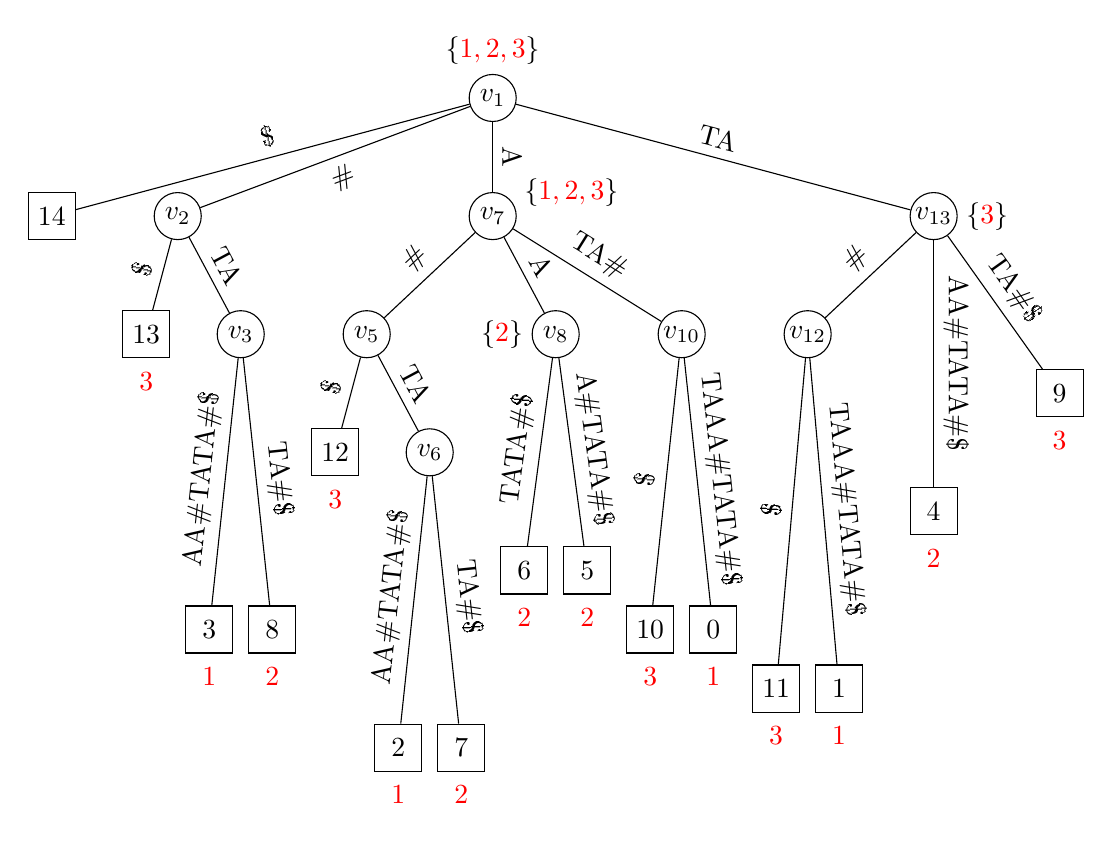
\begin{tikzpicture}[x={(4mm, 0mm)}, y={(0mm, 15mm)}]
  \tikzstyle{vertex}=[draw, minimum size=17pt, inner sep=0pt]

\node[vertex, circle] (v1) at (1, 0) {$v_1$};
\node (l1) at (1, 0.4) {$\{{\color{red}1,2,3}\}$};

\node[vertex, circle] (v2) at (-9, -1) {$v_2$};
\draw (v1) -- (v2) node[below, sloped, pos=0.5] {\#};

\node[vertex, circle] (v3) at (-7, -2) {$v_3$};
\draw (v2) -- (v3) node[above, sloped, pos=0.5] {TA};

\node[vertex, circle] (v7) at (1, -1) {$v_7$};
\node (l7) at (3.5, -0.8) {$\{{\color{red}1,2,3}\}$};
\draw (v1) -- (v7) node[above, sloped, pos=0.5] {A};

\node[vertex, circle] (v5) at (-3, -2) {$v_5$};
\draw (v7) -- (v5) node[above, sloped, pos=0.5] {\#};

\node[vertex, circle] (v6) at (-1, -3) {$v_6$};
\draw (v5) -- (v6) node[above, sloped, pos=0.5] {TA};

\node[vertex, circle] (v8) at (3, -2) {$v_8$};
\node (l8) at (1.3, -2) {$\{{\color{red}2}\}$};
\draw (v7) -- (v8) node[above, sloped, pos=0.5] {A};

\node[vertex, circle] (v10) at (7, -2) {$v_{10}$};
\draw (v7) -- (v10) node[above, sloped, pos=0.5] {TA\#};

\node[vertex, circle] (v13) at (15, -1) {$v_{13}$};
\node (l13) at (16.7, -1) {$\{{\color{red}3}\}$};
\draw (v1) -- (v13) node[above, sloped, pos=0.5] {TA};

\node[vertex, circle] (v12) at (11, -2) {$v_{12}$};
\draw (v13) -- (v12) node[above, sloped, pos=0.5] {\#};

\node[vertex] (s14) at (-13, -1) {$14$};
\draw (v1) -- (s14) node[above, sloped, pos=0.5] {\$};

\node[vertex] (s13) at (-10, -2) {$13$};
\node (d13) at (-10, -2.4) {${\color{red}3}$};
\draw (v2) -- (s13) node[above, sloped, pos=0.5] {\$};

\node[vertex] (s3) at (-8, -4.5) {$3$};
\node (d3) at (-8, -4.9) {${\color{red}1}$};
\draw (v3) -- (s3) node[above, sloped, pos=0.5] {AA\#TATA\#\$};

\node[vertex] (s8) at (-6, -4.5) {$8$};
\node (d8) at (-6, -4.9) {${\color{red}2}$};
\draw (v3) -- (s8) node[above, sloped, pos=0.5] {TA\#\$};

\node[vertex] (s12) at (-4, -3) {$12$};
\node (d12) at (-4, -3.4) {${\color{red}3}$};
\draw (v5) -- (s12) node[above, sloped, pos=0.5] {\$};

\node[vertex] (s2) at (-2, -5.5) {$2$};
\node (d2) at (-2, -5.9) {${\color{red}1}$};
\draw (v6) -- (s2) node[above, sloped, pos=0.5] {AA\#TATA\#\$};

\node[vertex] (s7) at (0, -5.5) {$7$};
\node (d7) at (0, -5.9) {${\color{red}2}$};
\draw (v6) -- (s7) node[above, sloped, pos=0.5] {TA\#\$};

\node[vertex] (s6) at (2, -4) {$6$};
\node (d6) at (2, -4.4) {${\color{red}2}$};
\draw (v8) -- (s6) node[above, sloped, pos=0.5] {TATA\#\$};

\node[vertex] (s5) at (4, -4) {$5$};
\node (d5) at (4, -4.4) {${\color{red}2}$};
\draw (v8) -- (s5) node[above, sloped, pos=0.5] {A\#TATA\#\$};

\node[vertex] (s10) at (6, -4.5) {$10$};
\node (d10) at (6, -4.9) {${\color{red}3}$};
\draw (v10) -- (s10) node[above, sloped, pos=0.5] {\$};

\node[vertex] (s0) at (8, -4.5) {$0$};
\node (d0) at (8, -4.9) {${\color{red}1}$};
\draw (v10) -- (s0) node[above, sloped, pos=0.5] {TAAA\#TATA\#\$};

\node[vertex] (s11) at (10, -5) {$11$};
\node (d11) at (10, -5.4) {${\color{red}3}$};
\draw (v12) -- (s11) node[above, sloped, pos=0.5] {\$};

\node[vertex] (s1) at (12, -5) {$1$};
\node (d1) at (12, -5.4) {${\color{red}1}$};
\draw (v12) -- (s1) node[above, sloped, pos=0.5] {TAAA\#TATA\#\$};

\node[vertex] (s4) at (15, -3.5) {$4$};
\node (d4) at (15, -3.9) {${\color{red}2}$};
\draw (v13) -- (s4) node[above, sloped, pos=0.5] {AA\#TATA\#\$};

\node[vertex] (s9) at (19, -2.5) {$9$};
\node (d9) at (19, -2.9) {${\color{red}3}$};
\draw (v13) -- (s9) node[above, sloped, pos=0.5] {TA\#\$};

\end{tikzpicture}

    \caption{The generalized suffix tree for concatenation $C = \texttt{ATA\#TAAA\#TATA\#\$}$. The red numbers on the leaves are the document array. The red marks on the inner vertices show the lowest common ancestor of two equal elements in the document array (as in document listing in Section~\ref{sec:documentListing}).}
    \label{fig:singleTermFrequencySuffixTree}
  \end{figure}

  In the next step the nodes need to be numbered. For each inner node~$v$ assign it the identifier $\id{id}(v)$ which is the index of the rightmost leaf in the leftmost subtree of~$v$ plus~$1$. This numbering has the following properties:
  \begin{enumerate}
    \item $\id{id}(v) \neq \id{id}(w)$ for all $v \neq w$. To show that this is true, we need to distinguish two cases: Assume $\proc{LCA}(v,w) \not\in \{v,w\}$. Then they have disjoint subtrees, so they get a different id. If however $\proc{LCA}(v,w) \in \{v,w\}$, then w.l.o.g. $v$ is in $w$'s subtree. But if they got the same id, then $v$ could have at most one child. If it had none, it is a leaf and would not be numbered. If it had exactly one, it would not even be part of the suffix tree.
    \item $\id{id}(v) \in [1,n]$ for all $v$. However, not all numbers from $[1,n]$ must appear as ids.
    \item $\id{id}(v) \in [\id{lb}(v), \id{rb}(v)]$, where $\id{lb}(v)$ and $\id{rb}(v)$ are the indices of the leftmost and rightmost leaves in $v$'s subtree ($[\id{lb}(v),\id{rb}(v)]$ is $v$'s suffix array interval).
  \end{enumerate}

  Next we connect each document id~$i$ at some node~$v_x$ to the closest ancestor~$_y$ that also contains document id~$i$ as shown in Figure~\ref{fig:singleTermFrequencySuffixTreeDocumentArrows}. This allows the following observations:
  \begin{itemize}
    \item The subset of nodes marked with document id $i$ correspond to the vertices of the suffix tree of document $i$.
    \item Document id $i$ occurs at most $n_i$ times in the leaves of the generalized suffix tree and therefore at most $n_i - 1$ times as an inner node. Summing up, this gives a total of at most $2n - N$ document labels in the whole \id{GST}.
  \end{itemize}

  \begin{figure}[htb]
    \centering
    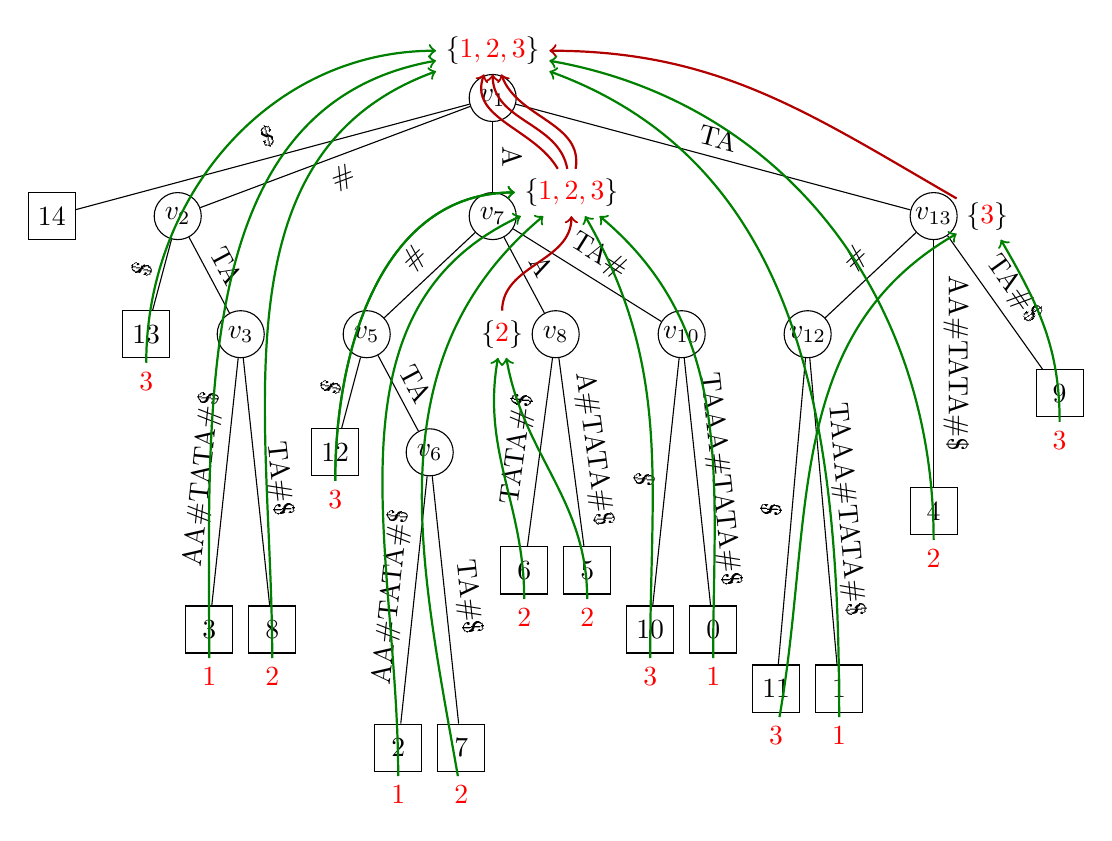
\begin{tikzpicture}[x={(4mm, 0mm)}, y={(0mm, 15mm)}]
  \tikzstyle{vertex}=[draw, minimum size=17pt, inner sep=0pt]

\node[vertex, circle] (v1) at (1, 0) {$v_1$};
\node (l1) at (1, 0.4) {$\{{\color{red}1,2,3}\}$};

\node[vertex, circle] (v2) at (-9, -1) {$v_2$};
\draw (v1) -- (v2) node[below, sloped, pos=0.5] {\#};

\node[vertex, circle] (v3) at (-7, -2) {$v_3$};
\draw (v2) -- (v3) node[above, sloped, pos=0.5] {TA};

\node[vertex, circle] (v7) at (1, -1) {$v_7$};
\node (l7) at (3.5, -0.8) {$\{{\color{red}1,2,3}\}$};
\draw (v1) -- (v7) node[above, sloped, pos=0.5] {A};

\node[vertex, circle] (v5) at (-3, -2) {$v_5$};
\draw (v7) -- (v5) node[above, sloped, pos=0.5] {\#};

\node[vertex, circle] (v6) at (-1, -3) {$v_6$};
\draw (v5) -- (v6) node[above, sloped, pos=0.5] {TA};

\node[vertex, circle] (v8) at (3, -2) {$v_8$};
\node (l8) at (1.3, -2) {$\{{\color{red}2}\}$};
\draw (v7) -- (v8) node[above, sloped, pos=0.5] {A};

\node[vertex, circle] (v10) at (7, -2) {$v_{10}$};
\draw (v7) -- (v10) node[above, sloped, pos=0.5] {TA\#};

\node[vertex, circle] (v13) at (15, -1) {$v_{13}$};
\node (l13) at (16.7, -1) {$\{{\color{red}3}\}$};
\draw (v1) -- (v13) node[above, sloped, pos=0.5] {TA};

\node[vertex, circle] (v12) at (11, -2) {$v_{12}$};
\draw (v13) -- (v12) node[above, sloped, pos=0.5] {\#};

\node[vertex] (s14) at (-13, -1) {$14$};
\draw (v1) -- (s14) node[above, sloped, pos=0.5] {\$};

\node[vertex] (s13) at (-10, -2) {$13$};
\node (d13) at (-10, -2.4) {${\color{red}3}$};
\draw (v2) -- (s13) node[above, sloped, pos=0.5] {\$};

\node[vertex] (s3) at (-8, -4.5) {$3$};
\node (d3) at (-8, -4.9) {${\color{red}1}$};
\draw (v3) -- (s3) node[above, sloped, pos=0.5] {AA\#TATA\#\$};

\node[vertex] (s8) at (-6, -4.5) {$8$};
\node (d8) at (-6, -4.9) {${\color{red}2}$};
\draw (v3) -- (s8) node[above, sloped, pos=0.5] {TA\#\$};

\node[vertex] (s12) at (-4, -3) {$12$};
\node (d12) at (-4, -3.4) {${\color{red}3}$};
\draw (v5) -- (s12) node[above, sloped, pos=0.5] {\$};

\node[vertex] (s2) at (-2, -5.5) {$2$};
\node (d2) at (-2, -5.9) {${\color{red}1}$};
\draw (v6) -- (s2) node[above, sloped, pos=0.5] {AA\#TATA\#\$};

\node[vertex] (s7) at (0, -5.5) {$7$};
\node (d7) at (0, -5.9) {${\color{red}2}$};
\draw (v6) -- (s7) node[above, sloped, pos=0.5] {TA\#\$};

\node[vertex] (s6) at (2, -4) {$6$};
\node (d6) at (2, -4.4) {${\color{red}2}$};
\draw (v8) -- (s6) node[above, sloped, pos=0.5] {TATA\#\$};

\node[vertex] (s5) at (4, -4) {$5$};
\node (d5) at (4, -4.4) {${\color{red}2}$};
\draw (v8) -- (s5) node[above, sloped, pos=0.5] {A\#TATA\#\$};

\node[vertex] (s10) at (6, -4.5) {$10$};
\node (d10) at (6, -4.9) {${\color{red}3}$};
\draw (v10) -- (s10) node[above, sloped, pos=0.5] {\$};

\node[vertex] (s0) at (8, -4.5) {$0$};
\node (d0) at (8, -4.9) {${\color{red}1}$};
\draw (v10) -- (s0) node[above, sloped, pos=0.5] {TAAA\#TATA\#\$};

\node[vertex] (s11) at (10, -5) {$11$};
\node (d11) at (10, -5.4) {${\color{red}3}$};
\draw (v12) -- (s11) node[above, sloped, pos=0.5] {\$};

\node[vertex] (s1) at (12, -5) {$1$};
\node (d1) at (12, -5.4) {${\color{red}1}$};
\draw (v12) -- (s1) node[above, sloped, pos=0.5] {TAAA\#TATA\#\$};

\node[vertex] (s4) at (15, -3.5) {$4$};
\node (d4) at (15, -3.9) {${\color{red}2}$};
\draw (v13) -- (s4) node[above, sloped, pos=0.5] {AA\#TATA\#\$};

\node[vertex] (s9) at (19, -2.5) {$9$};
\node (d9) at (19, -2.9) {${\color{red}3}$};
\draw (v13) -- (s9) node[above, sloped, pos=0.5] {TA\#\$};


  \draw[green!50!black, thick, ->] (d13) to[out=90, in=180] (l1);
  \draw[green!50!black, thick, ->] (d3) to[out=90, in=190] (l1);
  \draw[green!50!black, thick, ->] (d8) to[out=90, in=200] (l1);
  \draw[green!50!black, thick, ->] (d12) to[out=90, in=180] (l7);
  \draw[green!50!black, thick, ->] (d2) to[out=90, in=205] (l7);
  \draw[green!50!black, thick, ->] (d7) to[out=100, in=220] (l7);
  \draw[green!50!black, thick, ->] (d12) to[out=90, in=180] (l7);
  \draw[green!50!black, thick, ->] (d6) to[out=90, in=260] (l8);
  \draw[green!50!black, thick, ->] (d5) to[out=90, in=280] (l8);
  \draw[red!70!black, thick, ->] (l8) to[out=90, in=270] (l7);
  \draw[red!70!black, thick, ->] (l7) to[out=120, in=250] (l1);
  \draw[red!70!black, thick, ->] (l7) to[out=100, in=270] (l1);
  \draw[red!70!black, thick, ->] (l7) to[out=80, in=290] (l1);
  \draw[red!70!black, thick, ->] (l13) to[out=150, in=0] (l1);
  \draw[green!50!black, thick, ->] (d10) to[out=90, in=300] (l7);
  \draw[green!50!black, thick, ->] (d0) to[out=90, in=320] (l7);
  \draw[green!50!black, thick, ->] (d11) to[out=80, in=210] (l13);
  \draw[green!50!black, thick, ->] (d1) to[out=90, in=340] (l1);
  \draw[green!50!black, thick, ->] (d4) to[out=90, in=350] (l1);
  \draw[green!50!black, thick, ->] (d9) to[out=90, in=300] (l13);
\end{tikzpicture}

    \caption{The suffix tree from Figure~\ref{fig:singleTermFrequencySuffixTree} with added arrows between document ids. The red arrows have weight at least $2$.}
    \label{fig:singleTermFrequencySuffixTreeDocumentArrows}
  \end{figure}

  We now have the index to answer queries. Consider a query $q$. We need to find the locus for $q$. Again this is the first node $v$, such that the path to $v$ is prefixed by $q$. Then we observe:
  \begin{itemize}
    \item Per document $i$ there is at most one arrow leaving $v$'s subtree upwards. For each of these pointers we associate a weight: For a pointer of document id $i$, the weight is equal to the number of times document $i$ appears in the subtree of $v$.
    \item The pointer of document $i$ leaving the locus $v$ has the biggest weight among all pointers for document $i$ in $v$'s subtree.
    \item Enumerating all the pointers leaving $v$'s subtree is equivalent to document listing. Top-$k$ frequency corresponds to retrieving the $k$ heaviest pointers (and respectively their corresponding documents).
  \end{itemize}

  We will now describe how the problem to find the heaviest pointers can be mapped to an orthogonal range queries problem. We already know of efficient solutions for that.
  
  From now on we will only consider arrows with a weight at least ~$2$. In Figure~\ref{fig:singleTermFrequencySuffixTreeDocumentArrows} this is the red subset of the arrows. All other (green) arrows correspond to documents where a query appears only once. If our method considering only the heavy arrows returns less than $k$ documents, we can use the classical document listing structure to find more documents.

  Each pointer is assigned a $(x,y)$-coordinate. For this we need a bitvector~$H$ similar to the one used for document listing. It is generated by first writing~$n$~$1$s and then inserting a~$0$ right before the $i$-th~$1$ per upward arrow leaving node~$v_i$. Obviously the~$0$s in~$H$ correspond to the pointers and the pointer corresponding to the~$i$-th~$0$ gets~$x$-coordinate~$i$. The~$y$-coordinate is the depth of the target node of the pointer. In our example we get the values in Table~\ref{tbl:topKPointerCoordinates}. The points are plotted into a grid in Figure~\ref{fig:singleTermFrequencyPlot}.
  \begin{table}[htb]
    \centering
    \begin{tabular}{rcl}
      $H$           & $=$ & \texttt{1~1~1~1~1~1~0~0~0~1~0~1~1~1~1~1~0~1~1~1} \\
      $\mathcal{D}$ & $=$ & \texttt{~~~~~~~~~~~~1~2~3~~~2~~~~~~~~~~~3} \\
      $x$           & $=$ & \texttt{~~~~~~~~~~~~0~1~2~~~3~~~~~~~~~~~4} \\
      $y$           & $=$ & \texttt{~~~~~~~~~~~~0~0~0~~~1~~~~~~~~~~~0} \\
      $w$           & $=$ & \texttt{~~~~~~~~~~~~2~3~2~~~2~~~~~~~~~~~2}
    \end{tabular}
    \caption{The mapping of pointers to coordinates for the example suffix tree in Figure~\ref{fig:singleTermFrequencySuffixTreeDocumentArrows}.}
    \label{tbl:topKPointerCoordinates}
  \end{table}

  \begin{figure}[htb]
    \centering
    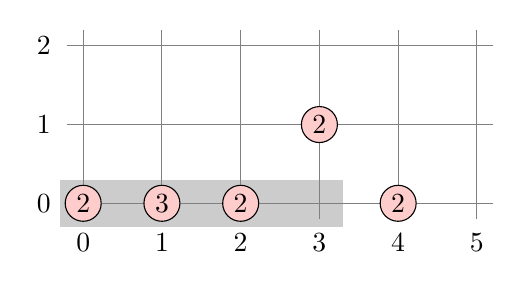
\begin{tikzpicture}
  \tikzstyle{vertex}=[draw, minimum size=13pt, inner sep=0pt]

  \fill[black!20!white] (-0.3, -0.3) -- (3.3, -0.3) -- (3.3, 0.3) -- (-0.3, 0.3) -- cycle;

  \foreach \x in {0, 1, ..., 5} {
    \draw[black!50!white] (\x, -0.2) -- (\x, 2.2);
    \node (x\x) at (\x, -0.5) {$\x$};
  }
  \foreach \y in {0, 1, 2} {
    \draw[black!50!white] (-0.2, \y) -- (5.2, \y);
    \node (y\y) at (-0.5, \y) {$\y$};
  }

  \node[vertex, circle, fill=red!20!white] (p1) at (0, 0) {$2$};
  \node[vertex, circle, fill=red!20!white] (p2) at (1, 0) {$3$};
  \node[vertex, circle, fill=red!20!white] (p3) at (2, 0) {$2$};
  \node[vertex, circle, fill=red!20!white] (p4) at (3, 1) {$2$};
  \node[vertex, circle, fill=red!20!white] (p5) at (4, 0) {$2$};
\end{tikzpicture}

    \caption{The points corresponding to the pointers with weight at least two plotted into a $2$-dimensional grid. The shaded area corresponds to the query range $[0, 3] \times [0, 0]$}
    \label{fig:singleTermFrequencyPlot}
  \end{figure}

  Assume the query $q = \texttt{A}$ and \proc{Backward Search} returns a suffix array interval $[l,r] = [4,10]$ for it. These are the positions of the leftmost and rightmost leaves descending form locus $v = v_7$ (note that $v$ is not computed and not known). Via two select queries interval $[l,r]$ can be mapped to an interval $[l',r'] = [0,3]$ in the $x$-coordinates. We extract the positions of the zeros in $H$ in $[l,r]$ as shown in Algorithm~\ref{alg:singleTermFrequencyMapInterval}. For the $y$-coordinates the lower bound is always $0$. For the upper bound we remember that the $y$-coordinate of the plotted points is the depth of the target node and that we only want to find arrows ending above the locus. Therefore we can take the length $\vert q \vert - 1$ as the upper $y$-coordinate. We reduced the query operation to a $3$-sided range query for the $k$ heaviest points in $[l', r'] \times [0, \vert q \vert - 1]$. This can be solved with the known range query methods from Section~\ref{chp:rangeQueries}. For our example the query range is shown shaded in Figure~\ref{fig:singleTermFrequencyPlot}.

  \begin{algorithm}[htb]
    \begin{codebox}
      \Procname{$\proc{Map-Interval}([l,r])$}
      \li $[l', r'] \gets [0, -1]$
      \li \If $l > 0$
          \Then
      \li   $l' \gets \proc{Select}_1(l - 1, H) - (l - 1)$
          \End
      \li \If $r > 0$
          \Then
      \li   $r' \gets \proc{Select}_1(r - 1, H) - r$
          \End
      \li \Return $[l', r']$
    \end{codebox}
    \caption{Maps a suffix array interval $[l,r]$ to an $x$-interval $[l',r']$.}
    \label{alg:singleTermFrequencyMapInterval}
  \end{algorithm}
\end{Proof}

At last, an optimal solution is known but is not covered in this document.

\begin{Theorem}
  The top-$k$ documents can be found in time $\mathcal{O}(m + k)$ query time in $\mathcal{O}(n \log n)$ bits space (Navarro \& Nekrich \cite{Navarro2012} based on framework by Hon \cite{Hon2014}).
\end{Theorem}

